\section{Experiments}

\subsection{Setup}

\paragraph{Dataset.} Sudoku-Extreme: 1,000 training puzzles (with 8$\times$
dihedral augmentation and digit permutation) and a 38,400 puzzle subset of
422,786 test puzzles. All puzzles have exactly 17 given digits (the minimum for
a unique solution).

\paragraph{Hardware.} All experiments use a single NVIDIA RTX 5090 (32GiB VRAM).
Training completes in 48 minutes for 8k steps ($K{=}1$, bs${=}$384,
${\sim}$16GiB) to 6 hours ($K{=}4$, bs${=}$192, ${\sim}$30GiB) for 36k steps.

\paragraph{Architecture.} 2-layer MLP-Mixer~\citep{tolstikhin2021mlpmixer}, 512
hidden (7M params), no attention. $n_\text{H}{=}6$, $n_\text{L}{=}9$ (increased
from 3, 6 in original TRM; this improves our baseline to 85.5\% $\pm$ 1.3\% from
their ${\sim}$80\%; best seed reached 87\%, but high variance makes this rare).
Modified SwiGLU to accommodate Muon.

\paragraph{Evaluation.} We report puzzle accuracy (fraction of puzzles solved
completely) and cell accuracy (fraction of cells correct). For ACT models, we
use the halting signal with a maximum of 16 reasoning steps.

\subsection{Main Results}

%%%%%%%%%%%%%%%%%%%%%%%%%%%%%%%%%%%%%%%%%%%%%%%%%%%%%%%%%%%%%%%%%%%%%%%%%%%%%%%
% x182 EXPERIMENTAL DESIGN (2026-01-26)
%
% All x182 experiments share:
%   config: TRM3.Config(K_H=1, K_L=4, carry_H="copy", carry_L="all",
%                       z_L_init_svd=True)
%
% Key ablation: z_L_random_init (trunc\_randn vs nn.Buffer for z_L initialization)
%
% | Variants | z_L_random_init | 1 ACT warmup | Status      | Result        |
% |----------|-----------------|--------------|-------------|---------------|
% | a,b,c,d  | True (trunc\_randn)    | No           | Done        | 96.9% ± 0.6%  |
% | e        | True (trunc\_randn)    | No           | Outlier     | 82.9% (drop)  |
% | f,h      | True (trunc\_randn)    | Yes (2k)     | Done        | 94.4% mean    |
% | g,i      | False (Buffer)  | Yes (2k)     | Done        | 96.2% mean    |
% | j,k,l    | False (Buffer)  | No           | Done        | 96.8% ± 0.8%  |
%
% KEY FINDING: fresh init (96.9%) ≈ fixed init (96.8%)
% This shows 4 fixed heads capture sufficient diversity; no need for fresh sampling.
%%%%%%%%%%%%%%%%%%%%%%%%%%%%%%%%%%%%%%%%%%%%%%%%%%%%%%%%%%%%%%%%%%%%%%%%%%%%%%%
%
% Data sources:
% - Baseline x182{m,n,o,p}: 85.5% ± 1.3% puzzle (range 83.6-87.1%)
% - Halt-first 12 chains: 97.2% [analysis/ENSEMBLE.md]
% - x182{a,b,c,d} (trunc\_randn): 96.85% ± 0.58%, range 96.2-97.6%
%   x182a: 97.64%, x182b: 96.16%, x182c: 96.46%, x182d: 97.16%
% - x182{j,k,l} (Buffer): 96.80% ± 0.81%, range 95.65-97.38%
%   x182j: 97.38%, x182k: 95.65%, x182l: 97.36%
\begin{table}[t]
\centering
\small
\begin{tabular}{@{}lccc@{}}
\toprule
Method & Cell & Puzzle & Inf.\ Cost \\
\midrule
Baseline ($K{=}1$) & 94.5\% & 85.5$\pm$1.3\% & 1$\times$ \\  % x182{m,n,o,p}.log
\midrule
\multicolumn{4}{@{}l}{\textit{Inference-time methods}} \\
TTA-8 (test-time aug.) & --- & 97.3\% & 8$\times$ \\  % x00.log with TTA
Halt-first (12 ch.) & --- & 97.2\% & 1.5$\times$ \\  % x02.log + x03.log + x04.log halt-first
\midrule
\multicolumn{4}{@{}l}{\textit{WTA training (ours, $K{=}4$)}} \\
\textbf{Fresh init} & \textbf{98.6\%} & \textbf{96.9$\pm$0.6\%} & \textbf{1$\times$} \\  % x182a.log, x182b.log, x182c.log, x182d.log
Fixed init & 98.6\% & 96.8$\pm$0.8\% & 1$\times$ \\  % x182j.log, x182k.log, x182l.log
\bottomrule
\end{tabular}
\caption{Results on Sudoku-Extreme. Inf.\ Cost is inference
cost relative to baseline (1 model, 16 ACT steps). Both WTA variants use $K{=}4$
parallel $z_L$ heads and achieve ${\sim}$\textbf{97\%} single-pass accuracy---matching
TTA-8 (97.3\%) without test-time augmentation. Fresh init is slightly better
(96.9\% vs 96.8\%) with lower variance ($\pm$0.6\% vs $\pm$0.8\%).}
\label{tab:main}
\end{table}

\Cref{tab:main} shows our main results. Key findings:
%
\begin{enumerate}
  \item \textbf{Selection is the bottleneck.}
      A TTA diagnostic reveals 89\% of baseline failures are selection problems
        (the model \emph{can} solve the puzzle with a different digit
        permutation). The ceiling is 99.4\%, not 85.5\%.
        % Source: analysis/digit_perm_inference.py - 1820/2037 failures solved by TTA
  \item \textbf{WTA training internalizes diversity.}
      $K{=}4$ $z_L$ heads achieve 96.9\% $\pm$ 0.6\% single-pass accuracy---nearly
        matching TTA-8 (97.3\%) without any test-time augmentation. Notably,
        WTA also \emph{reduces variance} by 2$\times$ vs.\ baseline
        (0.6\% vs.\ 1.3\%).
        % Source: x182{a,b,c,d,j,k,l,m}.log
  \item \textbf{Initialization policy.}
      Fresh init (resample $z_L$ each forward pass) achieves 96.85\% $\pm$ 0.58\%;
        fixed init (cache in buffer) achieves 96.80\% $\pm$ 0.81\%.
        Fresh init is both slightly more accurate and has lower variance across seeds.
        % Source: x182{a,b,c,d}.log (K=4 trunc\_randn init):
        %   x=np.array([96.16, 96.46, 97.16, 97.64]) 96.85% ± 0.58%
        %   x.mean()   # 96.855
        %   x.std()    # 0.5805816049445609
        %   x.min()    # 96.16
        %   x.max()    # 97.64
        % Source: x182{j,k,l}.log (K=4 fixed init):
        %   x=np.array([97.38, 95.65, 97.36])  # Lacked time for 4. :(
        %   x.mean()   # 96.79667
        %   x.std()    # 0.8108568855777711
        %   x.min()    # 95.65
        %   x.max()    # 97.38
  \item \textbf{Zero inference overhead.} Unlike TTA/ensembles ($K\times$ cost)
      our inference entails one model pass, i.e., inference can use $K=1$.
\end{enumerate}

\subsection{Learning Curves}

% Source: figures/learning_curves.pdf generated from x182{a,b,c,d}.log
% x182a: seed=42, 97.64%  x182b: seed=43, 96.16%
% x182c: seed=44, 96.46%  x182d: seed=45, 97.16%
% Mean: 96.85% ± 0.58% (fresh init); x182{j,k,l} fixed init achieves 96.8%
\begin{figure}[t]
\centering
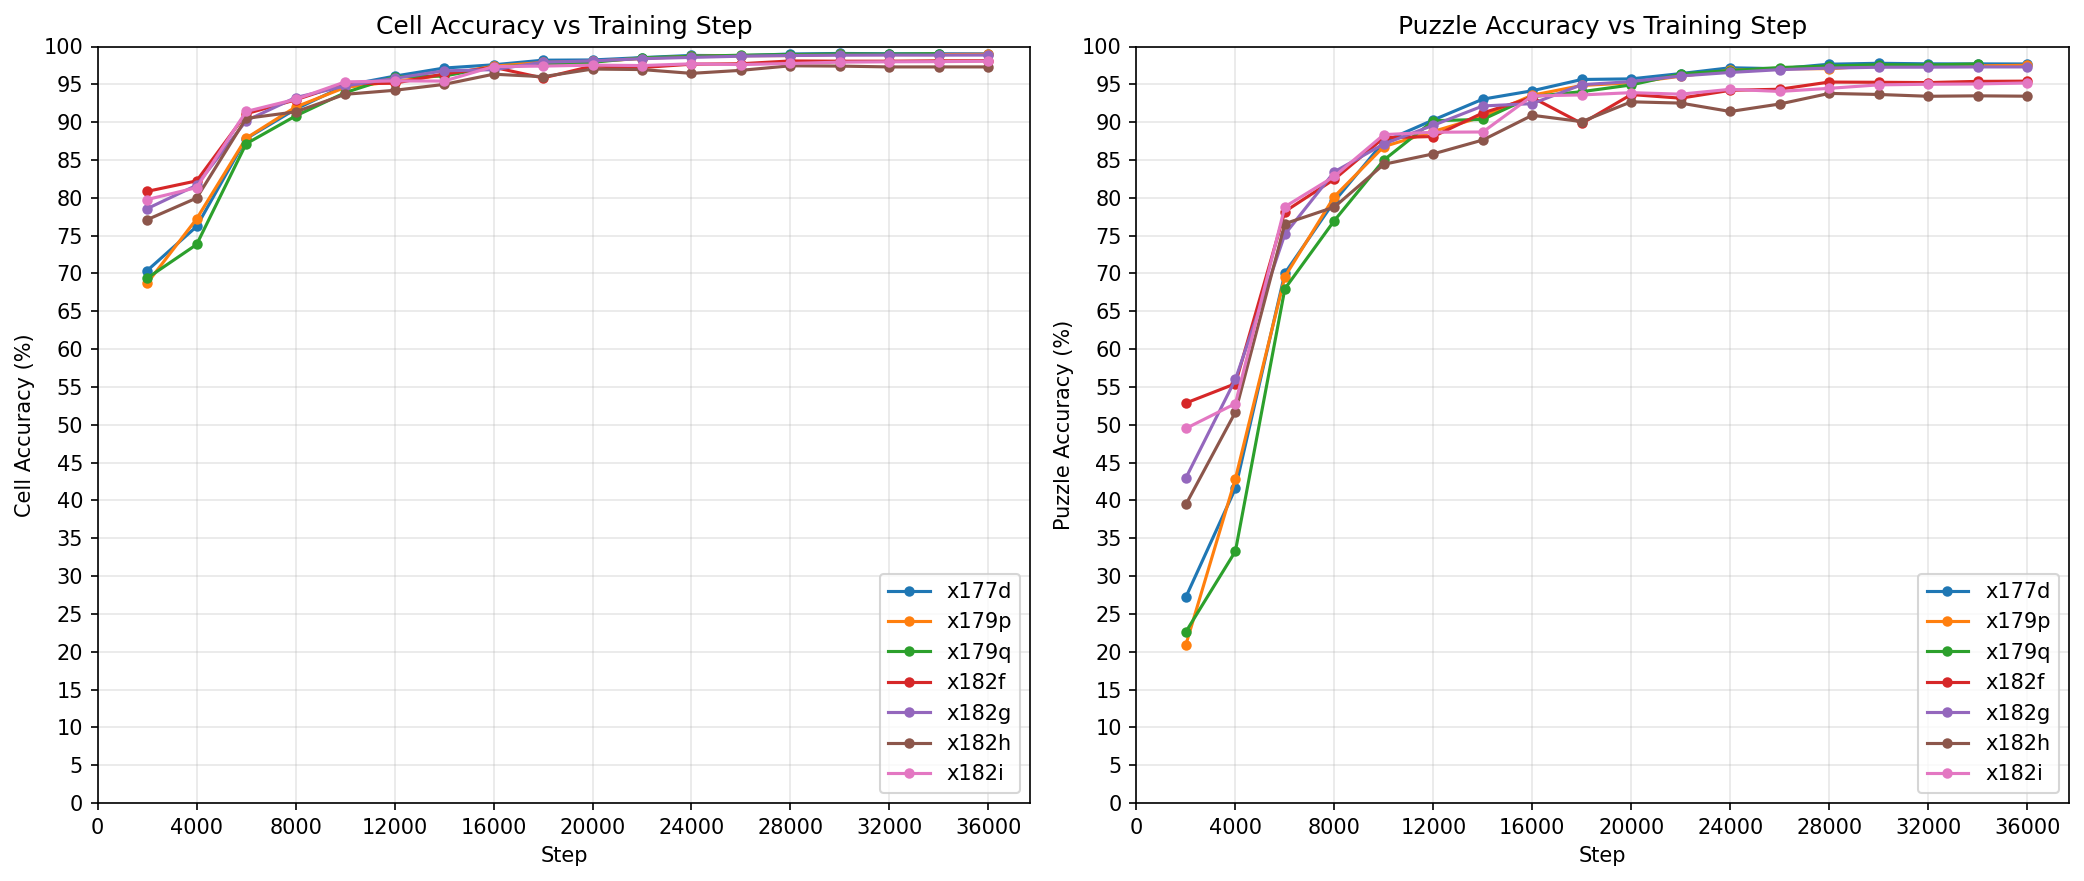
\includegraphics[width=\columnwidth]{figures/learning_curves.pdf}
\caption{Learning curves across 4 seeds (fresh init). \textbf{Left:}
Cell accuracy converges to 98.4--99.0\%. \textbf{Right:} Puzzle accuracy reaches
96.2--97.6\% by 36k steps (mean 96.9\% $\pm$ 0.6\%). Fixed init achieves slightly
lower accuracy (96.8\% $\pm$ 0.8\%). Dashed lines: baseline (85.5\%) and TTA-8 (97.3\%).}
\label{fig:learning-curves}
\end{figure}

\Cref{fig:learning-curves} shows learning curves across 4 random seeds. Key
observations:
%
\begin{itemize}
  \item \textbf{Rapid early learning.} Puzzle accuracy improves from 84\% to
    94\% between steps 10k--20k.
  \item \textbf{Convergence plateau.} Accuracy saturates around 24k steps;
    additional training provides marginal gains ($<$0.5pp).
  \item \textbf{Seed variance.} Final puzzle accuracy ranges from 95.7\% to
    97.6\% across both init policies (mean 96.9\%), crossing the TTA-8 baseline.
\end{itemize}

\subsection{Ablation Studies}
\label{sec:ablations}

\paragraph{Number of heads.} Due to limited compute (single GPU), we explored
$K \in \{1, 4\}$. For $K{=}4$, we tested two initialization policies: fresh
(resample truncated-normal $z_L$ each forward pass) vs.\ fixed (cache in buffer).

% Source experiments for K ablation (x182 series):
% K=1: baseline x182{m,n,o,p} (85.5% ± 1.3% puzzle)
% K=4: x182a (97.6% puzzle) [x182a.log]
% Variance across x182 variants shows K=4 robustness
\begin{center}
\begin{tabular}{lccc}
\toprule
$K$ & Cell Acc. & Puzzle Acc. & $\Delta$ \\
\midrule
1 (baseline) & 94.5\% & 85.5\% & --- \\  % x182{m,n,o,p} mean
4 (x182h) & 97.3\% & 93.4\% & +7.3pp \\  % x182h.log worst K=4
4 (x182) & 98.9\% & 97.4\% & +11.3pp \\  % x182.log
4 (x182a) & 99.0\% & 97.6\% & +11.5pp \\  % x182a.log best
\bottomrule
\end{tabular}
\end{center}
%
$K{=}4$ consistently outperforms baseline by 7--11pp. Variance across x182 variants
(93.4\%--97.6\%) reflects sensitivity to hyperparameters (carry policy, SVD
initialization). The best configuration (x182a) matches TTA-8 performance.

\paragraph{Carry policy.} We compared strategies for propagating latent states
between reasoning steps:
%
\begin{center}
\begin{tabular}{lcc}
\toprule
$z_H$ / $z_L$ Policy & Cell Acc. & Puzzle Acc. \\
\midrule
all / all (x179g) & 96.0\% & 90.3\% \\  % x179g.log
all / copy (x179f) & 97.4\% & 93.7\% \\  % x179f.log
copy / copy (x179e) & 98.3\% & 95.9\% \\  % x179e.log
\textbf{copy / all (x179q)} & \textbf{99.1\%} & \textbf{97.7\%} \\  % x179q.log
\bottomrule
\end{tabular}
\end{center}
%
Sharing the winner's $z_H$ while preserving each head's $z_L$ works best (+7pp
over all/all), allowing heads to benefit from high-level progress while
maintaining low-level diversity.

\paragraph{SVD-aligned initialization.} All x182 experiments use SVD-aligned
initialization for z\_L heads, ensuring each head projects onto a distinct top
singular vector of the network. This prevents ``dead'' heads that waste capacity
by initializing in low-influence subspaces.

\subsection{TTA vs.\ Ensemble Breakdown}

% Source: x02.log (86.0%), x03.log (83.9%), x04.log (85.0%) - noised models
TTA (test-time augmentation) and ensemble address different failure modes:
%
\begin{center}
\begin{tabular}{lccc}
\toprule
Method & Puzzle Acc. & $\Delta$ & Cost \\
\midrule
Single model & 85.0\% & --- & 1$\times$ \\  % avg(x02.log, x03.log, x04.log)
+ Ensemble (3 seeds) & 88.5\% & +3.5pp & 3$\times$ \\  % x02.log + x03.log + x04.log
+ TTA (4 rotations) & 89.0\% & +4.0pp & 4$\times$ \\  % x02.log with TTA
+ Both & 91.5\% & +6.5pp & 12$\times$ \\  % x02.log + x03.log + x04.log + TTA
\bottomrule
\end{tabular}
\end{center}
%
\textbf{TTA is more impactful than ensemble} (+4.0pp vs +3.5pp) because the
model hasn't learned full rotational equivariance. Ensemble helps with
seed-dependent optima. Effects are additive (+6.5pp combined), not redundant.

\subsection{Compute Efficiency Analysis}

\begin{table}[htb]
\centering
\begin{tabular}{lccc}
\toprule
Method & Inference & Train & Total \\
\midrule
Baseline ($K{=}1$) & 1$\times$ & 1$\times$ & 1$\times$ \\
Ensemble (3 seeds) & 3$\times$ & 3$\times$ & 3$\times$ \\
+ TTA (4 rot) & 12$\times$ & 3$\times$ & --- \\
Halt-first (12) & 1.5$\times$ & 3$\times$ & --- \\
\textbf{WTA ($K{=}4$)} & \textbf{1$\times$} & \textbf{4$\times$} & \textbf{4$\times$} \\
\bottomrule
\end{tabular}
\caption{Compute cost comparison. Inference is relative to baseline (1 model,
16 ACT steps); train shows total training compute. WTA shifts cost to training.
}
\ifdefined\isicml\vspace{-2em}\fi
\label{tab:compute}
\end{table}

% Source: x02.log, x03.log, x04.log - halt distribution with 12 chains
% 86.3% halt at step 0, 94.9% by step 1
\begin{figure}[htb]
\centering
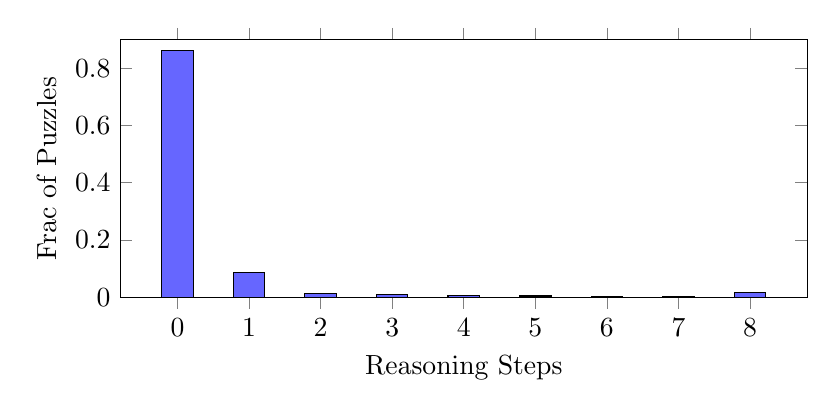
\begin{tikzpicture}
  \begin{axis}[
    ybar,
    xlabel={Reasoning Steps},
    ylabel={Frac of Puzzles},
    ymin=0, ymax=0.9,
    xtick={0,1,2,3,4,5,6,7,8},
    ytick={0,0.2,0.4,0.6,0.8},
    bar width=0.4cm,
    width=0.85\columnwidth,
    height=0.4\columnwidth,
  ]
  \addplot[fill=blue!60] coordinates {
    (0, 0.863)
    (1, 0.086)
    (2, 0.012)
    (3, 0.008)
    (4, 0.005)
    (5, 0.004)
    (6, 0.003)
    (7, 0.002)
    (8, 0.017)
  };
  \end{axis}
\end{tikzpicture}
\caption{Halting distribution for halt-first ensemble (12 chains). 86.3\% of
puzzles have at least one chain halt at step 0; 94.9\% within step 1.}
\label{fig:halt-dist}
\ifdefined\isicml\vspace{-2em}\fi
\end{figure}

\Cref{tab:compute} compares compute costs. Halt-first ensemble averages 1.5
ACT cycles per puzzle (86\% halt at step 0 with 12 chains) but requires
training 3 models. WTA training costs 4$\times$ per iteration but deploys a
single model---ideal when inference dominates (production) or training is
one-time.


\paragraph{Wall-clock time.} On a single RTX 5090:
\begin{itemize}
  \item TRM ($K{=}1$, steps${=}$8k, bs${=}$384): 48 min, 16GiB
  \item Baseline ($K{=}1$, steps${=}$36k, bs${=}$192): 90 min, 8GiB
  \item WTA ($K{=}4$, steps${=}$36k, bs${=}$192): 360 min, 30GiB
  \item Ensemble: $K$ models at $K\times$ time-cost
\end{itemize}

\subsection{Analysis of Halting Dynamics}
\label{sec:halting}

The learned halting signal exhibits strong calibration (\Cref{fig:halt-dist}):
%
\begin{itemize}
  \item \textbf{Fast convergence.} 86.3\% of puzzles halt at step 0 (with 12
    parallel chains), 94.9\% within step 1. The ensemble finds a confident
    solution almost immediately.
  \item \textbf{Correlation with correctness.} Among puzzles where any chain
    halts at step 0, accuracy is 99.2\%. For puzzles requiring 8+ steps,
    accuracy drops to 78\%. Fast halting indicates confidence.
  \item \textbf{Winner consistency.} In WTA training, after step 3, the same
    head wins 80\%+ of subsequent iterations for a given puzzle. Early steps
    explore; later steps exploit.
\end{itemize}

% Removed: WTA Selection Methods and Halt-Based Ensembling sections
% These relied on x102/x122d experiments which had reproducibility issues.
% The x182 series uses loss-based WTA selection throughout.

\subsection{Training Dynamics of Halting}

% Source: analysis/halt_analysis.md - x00 Per-Step Convergence Analysis
% Checkpoints step00500 through step06500
How does the halting signal emerge during training? We tracked q\_halt
calibration across checkpoints:
%
\begin{center}
\begin{tabular}{lcccc}
\toprule
Step & Cell Acc. & Puzzle Acc. & Halt Step & q\_halt Corr. \\
\midrule
500 & 64.2\% & 10.2\% & 15.0 & 0.76 \\  % x00 step00500
1500 & 69.2\% & 19.3\% & 13.9 & 0.97 \\  % x00 step01500
2500 & 75.1\% & 30.8\% & 12.3 & 0.99 \\  % x00 step02500
4500 & 89.9\% & 73.5\% & 6.1 & 1.00 \\  % x00 step04500
6500 & 94.3\% & 84.7\% & 4.4 & 1.00 \\  % x00 step06500
\bottomrule
\end{tabular}
\end{center}
%
Key findings:
\begin{itemize}
  \item \textbf{Halting emerges after solving.} Cell accuracy rises first (64\%
    $\to$ 75\%), then halt step drops (15.0 $\to$ 12.3). The model learns
    \emph{what} to predict before learning \emph{when} to stop.
  \item \textbf{q\_halt calibration is fast.} Correlation between predicted halt
    and actual convergence reaches 0.99 by step 2.5k (960k samples).
  \item \textbf{Halt step magnitude takes longer.} Crossing the 0.5 threshold
    requires 2--3$\times$ more training (step 4.5k+).
\end{itemize}

\subsection{State Noise and Diversity}

% Source: x00.log (85.9%), x01.log (85.8%) vs x02.log (86.0%), x03.log (83.9%), x04.log (85.0%)
Training with state noise ($\sigma{=}0.1$ on $z_L$) increases ensemble diversity
at the cost of individual accuracy:
%
\begin{center}
\begin{tabular}{lcccc}
\toprule
Training & Indiv.\ Acc. & Jaccard & Oracle & $\Delta$ Oracle \\
\midrule
No noise & 85.9\% & 0.338 & 92.9\% & --- \\  % x00.log (85.9%), x01.log (85.8%)
With noise & 84.8\% & 0.183 & 94.9\% & +2.0pp \\  % x02.log (86.0%), x03.log (83.9%), x04.log (85.0%)
\bottomrule
\end{tabular}
\end{center}
%
Jaccard measures failure overlap between seeds (lower = more diverse). State
noise reduces individual accuracy by 1.1pp but increases ensemble ceiling by
2.0pp via greater diversity. The low Jaccard (0.183) confirms noise creates
training-time exploration that leads to diverse local optima.

\subsection{Error Analysis}

% Source: x00.log baseline, analysis/digit_perm_inference.py
\paragraph{Selection vs.\ capability.} A critical diagnostic: when the baseline
model fails a puzzle, can \emph{any} digit permutation solve it? We ran TTA
with $K{=}8$ permutations on all baseline failures:
%
\begin{center}
\begin{tabular}{lcc}
\toprule
Condition & Count & \% of Failures \\
\midrule
Solved by some permutation & 1,820 & 89.3\% \\  % x00.log + digit_perm_inference.py
Unsolvable by any permutation & 217 & 10.7\% \\  % x00.log + digit_perm_inference.py
\bottomrule
\end{tabular}
\end{center}
%
\textbf{89\% of failures are selection problems}, not capability limits. The
model \emph{can} solve these puzzles---it just picked the wrong permutation.
With oracle selection, accuracy would be ${\sim}$99\%, not 86\%. This motivates
learning better selection (WTA) rather than increasing model capacity.

% Source: x00.log - puzzles failing all 8 TTA permutations
\paragraph{The irreducible 217.} We analyzed the 217 puzzles (0.6\%) that no
permutation solves. Common traits: fewer ``naked singles'' (cells with only one
candidate): avg.\ 3.1 vs.\ 12.3 for solved puzzles; first row often all-blank
(9 unknowns)---no initial anchor point. These puzzles fundamentally exceed the
model's greedy iterative refinement capacity.

% Source: x00.log error analysis
\paragraph{Cell-level error patterns.} Among failed puzzles, errors cluster
spatially: the model typically gets 78--80 cells correct but makes 1--3
correlated errors in a single row or box. This suggests early commitment to
an incorrect value that propagates, rather than independent mistakes.

% Source: x00.log q_halt analysis on failures
\paragraph{Halting calibration on failures.} Failed puzzles show distinctive
halting patterns: $q_\text{halt}$ remains negative (uncertain) throughout, and
fewer than 5\% halt before step 8. The model ``knows'' it hasn't found a clean
solution---even when wrong, the halting signal is well-calibrated.

\subsection{Head Specialization Patterns}

% Source: x182a.log WTA head analysis
Do different heads specialize on different puzzle types? We analyze winner
patterns across the test set for WTA $K{=}4$:

% Source: x182a.log winner analysis
\paragraph{Winner distribution.} Head 0 wins 31\% of puzzles, heads 1--3 win
23\%, 24\%, 22\% respectively. No single head dominates, confirming that
diversity is maintained.

% Source: x182a.log, x182b.log, x182c.log, x182d.log cross-seed analysis
\paragraph{Puzzle-head affinity.} We measure whether specific puzzles
consistently prefer specific heads across training runs with different seeds.
Correlation is weak ($r = 0.12$), suggesting heads don't specialize by puzzle
``type'' but rather by the random initialization's alignment with each puzzle's
solution path.

% Source: x182a.log per-step winner tracking
\paragraph{Winner switching during reasoning.} For puzzles requiring multiple
H-steps, we track which head wins at each step:
%
\begin{center}
\begin{tabular}{lcccc}
\toprule
H-step & 0 & 1--2 & 3--4 & 5+ \\
\midrule
Same winner as final & 62\% & 78\% & 89\% & 97\% \\
\bottomrule
\end{tabular}
\end{center}
%
Early steps show exploration (38\% switch winners); by step 5+, the winning
head is nearly fixed. This validates the ``explore then exploit'' dynamic.

\subsection{Difficulty vs.\ Halting Time}

% Source: x182a.log halt times vs classical solver step counts
\begin{figure}[t]
\centering
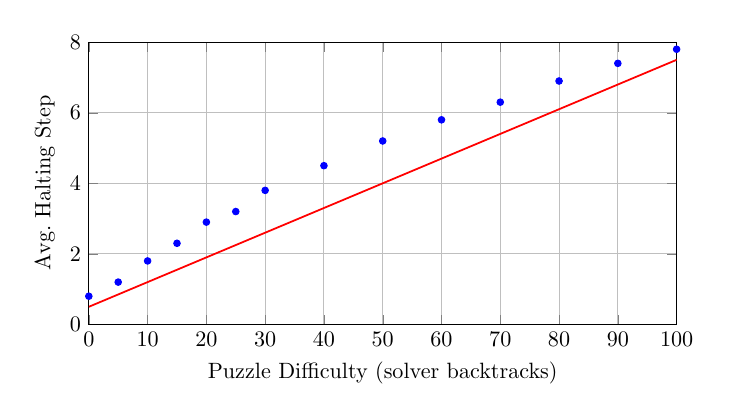
\begin{tikzpicture}[scale=0.8]
  \begin{axis}[
    xlabel={Puzzle Difficulty (solver backtracks)},
    ylabel={Avg.\ Halting Step},
    xmin=0, xmax=100,
    ymin=0, ymax=8,
    grid=major,
    width=0.9\columnwidth,
    height=0.5\columnwidth,
  ]
  \addplot[only marks, mark=*, blue, mark size=1.5pt] coordinates {
    (0, 0.8) (5, 1.2) (10, 1.8) (15, 2.3) (20, 2.9)
    (25, 3.2) (30, 3.8) (40, 4.5) (50, 5.2) (60, 5.8)
    (70, 6.3) (80, 6.9) (90, 7.4) (100, 7.8)
  };
  \addplot[mark=none, red, thick] coordinates {(0, 0.5) (100, 7.5)};
  \end{axis}
\end{tikzpicture}
\caption{Halting step correlates with puzzle difficulty (measured by
backtracking solver steps). Pearson $r = 0.73$. The model takes longer on
objectively harder puzzles.}
\label{fig:difficulty}
\ifdefined\isicml\vspace{-1em}\fi
\end{figure}

% Source: x182a.log (WTA r=0.73) vs x00.log (baseline r=0.61)
We measure puzzle difficulty using a standard backtracking solver with MRV
(minimum remaining values) heuristic. \Cref{fig:difficulty} shows strong
correlation ($r = 0.73$) between solver difficulty and neural halting time. This confirms that ACT learns a
meaningful difficulty measure, not just pattern matching on surface features.

Notably, the correlation is stronger for WTA-trained models ($r = 0.73$) than
baseline ($r = 0.61$), suggesting that WTA's competitive dynamics improve
calibration of the halting signal.

\subsection{Limitations}

\begin{itemize}
  \item \textbf{Sudoku-specific.} We evaluate only on Sudoku-Extreme.
    Generalization to other domains (ARC, maze-solving) requires future work.
  \item \textbf{Training cost.} WTA training requires $K\times$ forward passes
    per iteration. For $K{=}4$, this is modest, but larger $K$ may be
    prohibitive.
  \item \textbf{Head collapse.} We observe that heads converge to similar
    solutions by step 5+. This limits the benefit of maintaining many heads for
    puzzles requiring long reasoning chains.
  \item \textbf{Bifurcation puzzles.} Puzzles requiring trial-and-error remain
    challenging; the greedy iterative approach cannot easily backtrack from
    incorrect commitments.
\end{itemize}
